\documentclass[11pt, a4paper, twoside]{article} % o book si es muy extenso
\usepackage[utf8]{inputenc}
\usepackage[spanish]{babel}
\usepackage[T1]{fontenc}
\usepackage{lmodern} % Fuente moderna y legible
\usepackage{microtype} % Mejora el espaciado y la justificación
\usepackage{geometry} % Para controlar los márgenes
    \geometry{
        a4paper,
        top=2.5cm,
        bottom=2.5cm,
        left=3cm,
        right=2.5cm,
        headheight=14pt,
        footskip=1.2cm
    }
\usepackage{fancyhdr} % Para personalizar encabezados y pies de página
\usepackage{graphicx} % Para incluir imágenes
\usepackage{hyperref} % Para enlaces interactivos y metadatos
    \hypersetup{
        colorlinks=true,
        linkcolor=blue,
        filecolor=magenta,
        urlcolor=cyan,
        pdftitle={Título de tu Proyecto},
        pdfauthor={Tu Nombre},
        pdfsubject={Informe de Proyecto Escolar},
        pdfkeywords={Proyecto, Escuela, Informe, LaTeX},
        bookmarks=true,
        bookmarksopen=true,
        bookmarksnumbered=true,
    }
\usepackage{titlesec} % Para personalizar títulos de secciones
\usepackage{enumitem} % Para personalizar listas
\usepackage{setspace} % Para controlar el interlineado
    \onehalfspacing % Interlineado de 1.5 para mejor lectura
\usepackage{listings}
\usepackage{xcolor} % Asegúrate de tenerlo para los colores

% --- Configuración de listings para código ---
\definecolor{codegreen}{rgb}{0,0.6,0}
\definecolor{codegray}{rgb}{0.5,0.5,0.5}
\definecolor{codepurple}{rgb}{0.58,0,0.82}
\definecolor{backcolour}{rgb}{0.95,0.95,0.92}

\lstdefinestyle{mystyle}{
    backgroundcolor=\color{backcolour},
    commentstyle=\color{codegreen},
    keywordstyle=\color{magenta},
    numberstyle=\tiny\color{codegray},
    stringstyle=\color{codepurple},
    basicstyle=\ttfamily\footnotesize, % Fuente monoespaciada, tamaño pequeño
    breakatwhitespace=false,
    breaklines=true,
    captionpos=b,
    keepspaces=true,
    numbers=left, % Números de línea a la izquierda
    numbersep=5pt,
    showspaces=false,
    showstringspaces=false,
    showtabs=false,
    tabsize=2, % Tamaño de la tabulación
    frame=single, % Marco alrededor del código
    rulecolor=\color{black},
    frameround=tttt, % Esquinas redondeadas
    extendedchars=true, % Para caracteres extendidos (como 'ñ')
    literate={á}{{\'a}}1 {é}{{\'e}}1 {í}{{\'i}}1 {ó}{{\'o}}1 {ú}{{\'u}}1 {ñ}{{\~n}}1 % Para manejar tildes y eñes
}

\lstset{style=mystyle} % Aplicar el estilo por defecto
\usepackage{lastpage} % Para obtener el número total de páginas

% --- Personalización de títulos de secciones ---
\titleformat{\section}[block]
  {\normalfont\Large\bfseries\color{green!70!black}}
  {\thesection}{1em}{}
\titlespacing*{\section}
  {0pt}{1.5ex plus .1ex minus .2ex}{1ex plus .1ex}

\titleformat{\subsection}[block]
  {\normalfont\large\bfseries\color{blue!50!black}}
  {\thesubsection}{1em}{}
\titlespacing*{\subsection}
  {0pt}{1.5ex plus .1ex minus .2ex}{1ex plus .1ex}

% --- Configuración de encabezados y pies de página ---
\pagestyle{fancy}
\fancyhf{} % Borra los ajustes predeterminados
\fancyhead[RO,LE]{\thepage} % Número de página a la derecha en páginas impares, a la izquierda en pares
\fancyhead[LO]{\nouppercase{\rightmark}} % Título de la sección en la parte izquierda (páginas impares)
\fancyhead[RE]{\nouppercase{\leftmark}} % Título del capítulo en la parte derecha (páginas pares) (si usas 'book' o 'report')
\fancyfoot[C]{\textbf{Informe de Proyecto}} % Texto en el pie de página centrado
\renewcommand{\headrulewidth}{0.4pt} % Línea en el encabezado
\renewcommand{\footrulewidth}{0.4pt} % Línea en el pie de página

\begin{document}

\thispagestyle{empty} % Para que la primera página no tenga encabezado ni pie de página

\begin{titlepage}
    \begin{center}
        % --- Espacio superior ---
        \vspace*{2cm}

        % --- Logo del proyecto ---
        
\includegraphics[width=0.3\textwidth]{logo.png} % Ajusta el tamaño según tu logo
        \vspace{1cm}

        % --- Título del Proyecto ---
        {\color{green!80!black}\Huge\bfseries Compilador de HULK}\par
        \vspace{0.5cm}

        % --- Subtítulo (opcional) ---
        {\color{gray}\Large\itshape Un informe detallado sobre la implementaci\'on de un Compilador para el lenguaje HULK}\par
        \vspace{2cm}

        % --- Integrantes del Equipo ---
        {\Large\bfseries Integrantes:}\par
        \vspace{0.3cm} % Espacio entre "Integrantes:" y los nombres
        {\large  Kevin Marqu\'ez Vega}\par
        {\large  Javier Alejandro Gonz\'ales}\par
        {\large  Jos\'e Miguel Leyva}\par
        \vspace{1.5cm} % Espacio después de los nombres

        % --- Información del Curso/Asignatura ---
        {\large Asignatura: Compilaci\'on}\par
        {\large Universidad de La Habana}\par
        \vspace{0.5cm}

        % --- Fecha ---
        {\large \today}\par % Muestra la fecha actual
        \vfill % Empuja el contenido restante hacia abajo

        % --- Información adicional (opcional, por ejemplo, el semestre) ---
        {\small \color{gray!70!black} Semestre: Segundo Semestre | Tercer a\~no}\par

    \end{center}
\end{titlepage}

\clearpage
% ... (el resto de tu documento sigue aquí, como la tabla de contenido y las secciones)

\clearpage % Para empezar el contenido en una nueva página
% Aquí puedes incluir tu tabla de contenido, si la necesitas:
% \tableofcontents
% \clearpage

% --- Comienza el contenido de tu informe ---
\section{Introducción}
Para la aplicaci\'on de los conocimientos adquiridos en la asignatura de Compilaci\'on, se llev'o a cabo
la implementaci\'on y desarrollo de un compilador para el lenguaje HULK (Havana University Language for Kompilers)
utilizando \textbf{C} como lenguaje base.

El compilador se divide en 4 etapas fundamentales: An\'alisis l\'exico \textit{lexer}, An\'alisis sint\'actico \textit{parser}.
An\'alisis sem\'antico y Generaci\'on de c\'odigo. Cada etapa ser\'a explicada detalladamente en el presente informe.

\subsection{Flujo del Programa}
El flujo del programa sigue el camino de cualquier compilador est\'andar. Comienza en la funci\'on \textit{main()} dentro del script
\textbf{main.c} la cual se encarga de leer el contenido del archivo \textbf{script.hulk} convirtiendo el mismo cadena de texto. Dicha 
cadena es enviada al \textit{lexer} y \textit{parser} para los an\'alsis l\'exico y sint\'actico respectivamente. Si no ocurre ning\'un
error en las etapas descritas se generar\'a el \'Arbol de Sintaxis Abstracta (AST por sus siglas en ingl\'es). Posteriormente se comienza el
Chequeo Sem\'antico de las expresiones definidas en el archivo \textit{.hulk} y finalmente se llega a la etapa de Generaci\'on de C\'odigo,
en la cual se mostrar\'an los resultados de compilar un script del lenguaje HULK en un archivo generado llamado \textbf{output.ll} en 
la carpeta \textbf{build}.

\section{An\'alisis L\'exico: Lexer}
Para el an\'alisis l\'exico de cualquier lenguaje se necesitan, entre otras cosas, una definici\'on de \textbf{Token}. Un Token
es una cadena de car\'acteres que representa un s\'imbolo que se utiliza en el lenguaje, ejemplo : palabras claves, operadores, variables etc.
Se hizo un estudio a fondo del lenguaje \textbf{HULK} para obtener todos los tokens del mismo y preparar todo para comenzar el an\'alisis.

El lexer utilizado es el brindado por la librer\'ia \textit{Flex}, el cual es muy robusto y completo, facilitando el desarrollo
de esta etapa de la compilaci\'on. Dentro del mismo se definen las principales expresiones regulares que intervienen en el lengujae,
as\'i como la representaci\'on en string de cada token con su correspondiente valor de retorno.

\textit{Flex} proporciona un generador de lexer, el cual, conociendo las expresiones regulares que intervienen en el lenguaje, y una secuencia de
car\'acteres determina los tokens que participan en dicha cadena y los deja listos para el an\'alisis sint\'actico.

\section{An\'alisis Sint\'actico: Parser}
En el An\'alisis sint\'actico se hizo con el framework proporcionado por \textbf{Yacc}, el cual al obtener la gram\'atica, bien definida, 
crea un AST en funci\'on del conjunto de expresiones que se utilizaron en el programa Hulk. 

\subsection{La gram\'atica}
La definici\'on de la gramatica la puede encontrar en el archivo \texttt{parser.y} en la que se ve claramente las producciones. Debido a la comletitud
y complejidad del lenguaje se hizo necesario definir una gram\'atica que no fuera \textbf{LL1} para que todas las operaciones que intervienen en las expresiones
sean analizadas correctamente tanto por las tres primeras etapas como por la generaci\'on de c\'odigo intermedio.

\subsection{AST}
El AST es una parte fundamental del desarrollo de compiladores, por lo que se hizo necesario poder modelar el comportamiento del mismo. Como en el lenguaje C no
existe la programaci\'on orientada a objetos, es muy complicado simular la herencia y las clases abstractas, ambos conceptos facilitan la implementaci\'on y 
lectura de c\'odigo cuando se trata de estructuras arboreas.

Para representar el AST se defini\'o un nodo por cada tipo de expresi\'on definida en la gram\a'tica del lenguaje ejemplo: \texttt{LetInNode}, \texttt{FunctionDefinitionNode}, 
\texttt{LiteralNode} etc. Adem\'as con el objetivo de simular la herencia, cada nodo tiene entre sus propiedades un struct de tipo \textbf{ASTNode}, el cual contiene
todos los atributos que comparten los nodos del AST, como el tipo y el valor de retorno.

\begin{figure}[h!] 
    \centering
    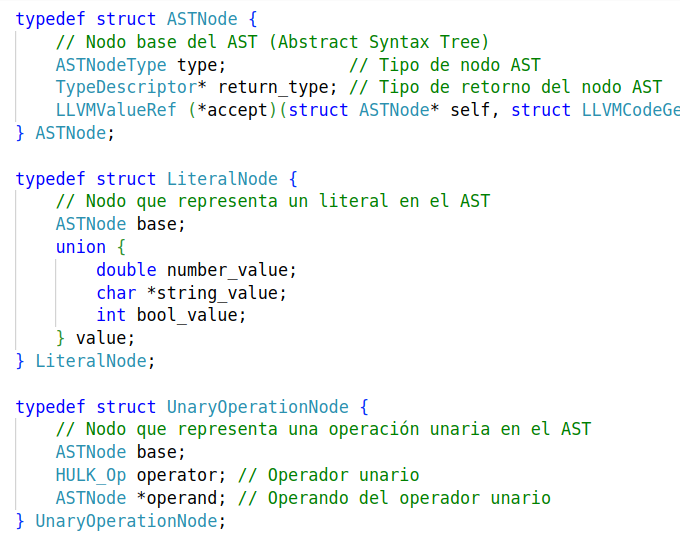
\includegraphics[width=0.8\textwidth]{ASTNode.png}
    \caption{Estructura de ASTNode} 
\end{figure}

\subsection{Flujo de Yacc}
Una vez definida la gram\'atica y el formato que tendr\'an los nodos del AST, se puede empezar a explicar el flujo de trabajo de Yacc. En el programa 
en C se tiene una funci\'on de creaci\'on por cada uno de los nodos anteriormente definidos. Dichas funciones son asociadas a las reglas de la gram\'atica
de esta forma se va construyendo el AST, dejando siempre como ra\'iz un nodo del tipo \texttt{ProgramNode} a partir del cual iniciar\'an los procesos que quedan.

\begin{figure}[h!] 
    \centering 
    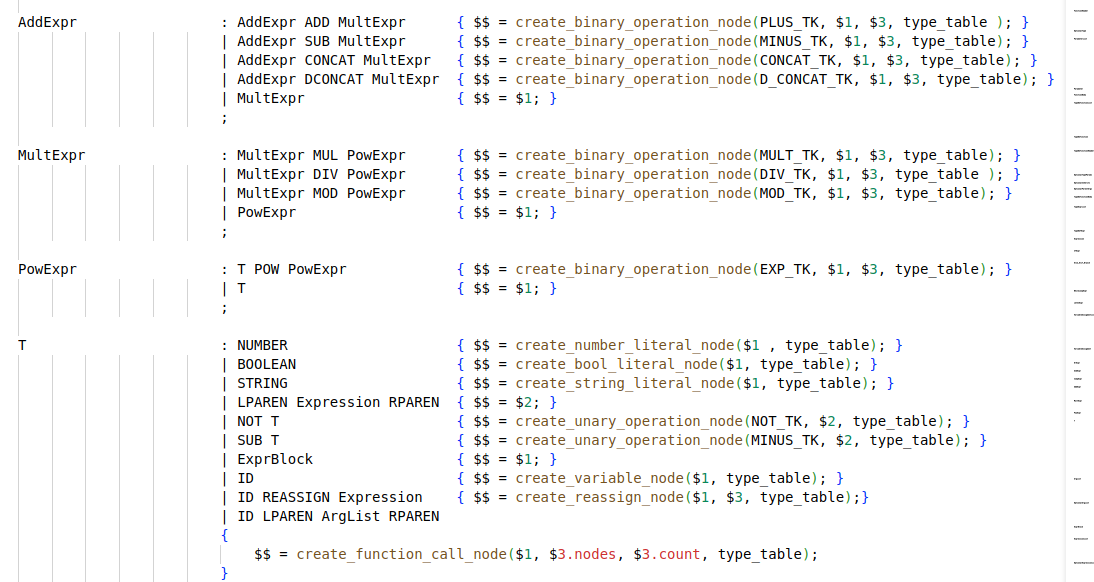
\includegraphics[width=0.8\textwidth]{CreacionAST.png}
    \caption{Algunos ejemplos de llamadas en funciones desde Yacc} 
\end{figure}

\begin{figure}[h!]
    \centering
    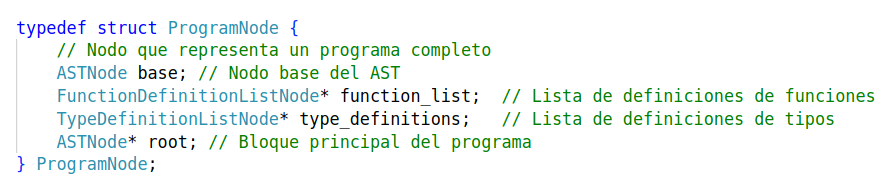
\includegraphics[width=0.8\textwidth]{ProgramNode.png}
    \caption{Estructura de ASTNode}
\end{figure}

\section{Chqueo Sem\'antico}
A partir de este momento comienza el chequeo sem\'antico, el cual est\'a implementado sin usar librer\'ias, bas\'andose en la definici\'on de nodos de AST mostrada
anteriormente. Se hace uso del \textbf{Patr\'on Visitor} para realizar esta tarea. El idea es hacer varios recorridos por el AST Generado dividiendo el trabajo en
varias etapas. La primera ser\'a para capturar todas las definiciones de funciones y creaci\'on de variables que se hallan realizado, la segunda para las definiciones 
de tipos y sus propiedades y finalmente para ver si el uso de las variables dentro de operaciones o funciones es el correcto de acuerdo a su tipo.

El compilador se pens\'o para la versi\'on de HULK de tipado est\'atico, \textit{Type-HULK} es decir, tanto para la definici\'on de funciones como para la de tipos
es necesario definir el tipo de cada uno de los par\'ametros. Esto ayuda en el momento de inferir el tipo de retorno de las funciones y ayuda a que no se hagan llamadas 
con los par\'ametros incorrectos, como por ejemplo \texttt{Factorial("5")}. 

Para llevar a cabo esta tarea, se definieron numerosas estructuras en C para manejar los contextos. Se tiene la struct \texttt{Symbol}, la cual se usa
para guardar todas las propiedades referidas al uso de variables y llamado de funciones. Una struct con el nombre de \texttt{SymbolTable}, que representa el contexto,
dicha tabla guarda la informaci\'on de todas aquellas variables y funciones que fueron definida en un contexto determinado. 

\subsection{Primera Etapa: Funciones}
Como se mencion\'o anteriormente en esta etapa se busca capturar todas las definciones de funciones que se realizaron en el script de HULK. Basicamente se recorre cada nodo
del AST hasta encontrar un \textbf{FunctionDefinitionNode}. Aclarar que en el lenguaje HULK no se pueden definir funciones dentro de otras funciones ni dentro de cualquier otro
nodo que implique la creaci\'on de un bloque de expresiones, por lo que este recorrido es posible y basta con analizar la \"Capa Superior\" del script.
Una vez encontradas todas las funciones se guardan en el Contexto global, permitiendo acceder a ellas desde cualquier punto del script de HULK.

\subsection{Segunda Etapa: Tipos}
Una vez guardadas todas las funciones en el Contexto global, se procede de manera similar para el analisis de tipo. Dentro de cada tipo se definir\'a un nuevo contexto, 
debido a que dentro del cuerpo de un tipo pueden existir propiedades y funciones, por tanto se guardan en un contexto propio que tienen los tipos nuevos definidos. 

\subsection{Tercera Etapa: Visita Sem\'antica}
Se implement\'o un struct \textbf{TypeDescriptor} en C para poder tener control de los tipos que intervienen en el lenguaje HULK as\'i como los tipos definidos por el usuario,
para estos \'ultimos se defini\'o la struct \textbf{TypeInfo}. El patr\'on visitor lo que har\'a es entrar en cada nodo del AST, los cuales tienen su propia forma de chequearse
e ir\'a retornando los TypeDescriptors correspondientes.

\begin{figure}[h!] 
    \centering 
    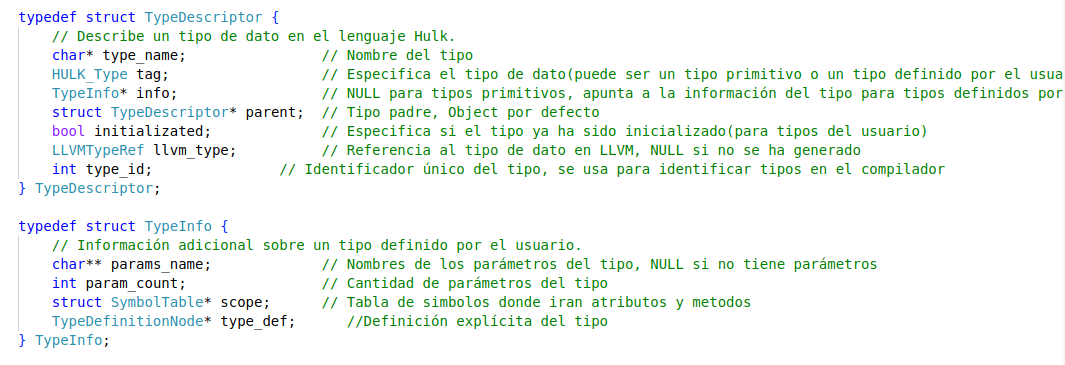
\includegraphics[width=0.8\textwidth]{Types.png}
    \caption{Type Descriptor y TypeInfo}
\end{figure}

\subsection{Declaraci\'on y uso de Variables}
Al declararse una variable en un programa de HULK, como bien se explic\'o anteriormente, se crea el s\'imbolo correspondiente y se guarda en el contexto en donde fue creada 
junto con su valor asignado. Si se encuentra el uso de la variable en alg\'un posterior a su definicio\'on, se chequea primera si en el contexto existe ya esa variable definida,
en HULK se pueden definir dos variables con el mismo nombre, al usar una dentro de un contexto, esta tomar\'a como valor el \'ultimo que se le asign\'o dentro del contexto actual,
o en un contexto superior. 

El patr\'on visitor, al llegar a una expresi\'on que indique el uso de una variable, deber\'a realizar las siguientes acciones: Chequear si dicha variable fue definida en el 
contexto actual o en uno superior y posteriormente analizar si su uso es correcto debido a su tipo de retorno.\\

\begin{lstlisting}[language=Go]
  let a = 10 in
    if (a >= 0)
    {
      print(a + 5);
    }
    else
    {
      let a = 11 in print(a);
    }
\end{lstlisting}

\subsection{Definici\'on y llamado de Funciones}
Las funciones siempre ser\'an definidas en el Contexto global del programa, como se explic\'o anteriormente, el tipado es est\'atico por lo que se debe especificar el tipo de cada 
par\'ametro de las funciones para poder declararlas. Como esto se conoce, es m\'as f\'acil determinar si las operaciones que se realizan dentro del cuerpo de una funci\'on 
tienen sem\'antica correcta.

Respecto al llamado de funciones, es sabido que en el HULK el tipo de retorno de una funci\'on es el mismo que el de su cuerpo, como el cuerpo de una funci\'on
puede ser un bloque de expresiones, entonces el tipo de retorno de una funci\'on es el de la \'ultima expresi\'on de su cuerpo. De esa forma al hacer algo como:\\

\begin{lstlisting}[language=Go]
function Sucesor(n : Number) => n + 1;
let a : Number = 3 in print(Square(a) + 4);
\end{lstlisting}

No ocurrir\'a ning\'un error sem\'antico, debido a que se especifica el tipo de dato del parametro \texttt{n} y es f\'acil determinar que la expresi\'on
\texttt{n + 1} es sem\'anticamente correcta y devuelve un tipo Number.

\subsection{Definici\'on de tipos y acceso a propiedades}
HULK es lenguaje con POO, por tanto se puede definir tipos nuevos en cualquier momento y utilizarlos en el programa

\end{document}